\section{Controller in time domain}

% State feedback controller
\subsection{State feedback controller}
As the reference is 0, we need not care about $k_r$, so we can fix it to 0.\par
However, if the reference was to change, we could compute $k_r$, it would be nice. Some tests of a change in reference will be performed in this report.\par
In a first time, we only need to compute the gain matrix $K$.\par
In order not to apply a gain on the wind force, our matrix K is as follows :
$$
K = \begin{pmatrix}
    0 & 0 & 0 & 0\\ 
    g_1 & g_2 & g_3 & g_4
\end{pmatrix}
$$
The new dynamic matrix of the closed-loop system is $A_{CL} = A - BK$. Let's determine the eigenvalues of that matrix.\par
As we have a matrix of dimension $4$, we will make the approximation of the dominant poles. Indeed, we have, from the previous matrix $A$, the eigenvalues :
\begin{align*}
    \lambda_1 &= \num{-0.0645 + 6.2824i}\\
    \lambda_2 &= \num{-0.0645 - 6.2824i}\\
    \lambda_3 &= \num{-1.6655 + 5.5285i}\\
    \lambda_4 &= \num{-1.6655 - 5.5285i}
\end{align*}
We can see that $\lambda_3$ and $\lambda_4$ are about $100$ times bigger than the last two, and so we do not need to work on them. Those two will therefore remain in $A_{CL}$.\par
Imposing that $(s - \lambda_3)(s - \lambda_4)$ is part of the decomposition, we get that the determinant of $A_{CL}$ is equal to :
$$
(s - \lambda_3)(s - \lambda_4)(s^2 + 2 \xi\omega_c s + \omega_c^2) = 0
$$
Since $\lambda_3$ and $\lambda_4$ are fixed, we only need to solve the equation of the second degree in $s$ in order to find the expressions of $\lambda_1$ and $\lambda_2$ as a function of $\xi$ and $\omega_c$.\par
The solutions of the equation are given by :
$$
\begin{cases}
    \lambda_1 = -\xi\omega_c - \omega_c\sqrt{\xi^2 - 1}\\
    \lambda_2 = -\xi\omega_c + \omega_c\sqrt{\xi^2 - 1}
\end{cases}
$$
The values of $\xi$ and $\omega_c$ will be determined by simulations in the following sections. When these have been fixed, we will obtain the values of the 4 poles of $A_{CL}$. Then we will just have to use the \texttt{place} function of Matlab to obtain the values $g_i$ of matrix $K$ associated with the eigenvalues.

% Observer
\subsection{Observer}
We need to compute the gain matrix $L$ :
$$
L = \begin{pmatrix}
    l_1\\
    l_2\\
    l_3\\
    l_4
\end{pmatrix}
$$
The new dynamic matrix is given by $A_{obs} = A - LC$.\par
As previously, we will keep the same two dominant eigenvalues and determine the two other via the same method we have used for $K$.\par
Imposing that $(s - \lambda_3)(s - \lambda_4)$ is part of the decomposition, we get that the determinant of $A_{obs}$ is equal to :
$$
(s - \lambda_3)(s - \lambda_4)(s^2 + 2 \xi\omega_c s + \omega_c^2) = 0
$$
Since $\lambda_3$ and $\lambda_4$ are fixed, we only need to solve the equation of the second degree in $s$ in order to find the expressions of $\lambda_1$ and $\lambda_2$ as a function of $\xi$ and $\omega_c$.\par
The solutions of the equation are given by :
$$
\begin{cases}
    \lambda_1 = -\xi\omega_c - \omega_c\sqrt{\xi^2 - 1}\\
    \lambda_2 = -\xi\omega_c + \omega_c\sqrt{\xi^2 - 1}
\end{cases}
$$
The poles of the observer are determined by taking the poles of the controller and moving them. To do this, the real parts of each pole are multiplied by a constant $\alpha$. In the case of poles $\lambda_1$ and $\lambda_2$, this amounts to multiplying $w_c$ by $\alpha$.\par
We finally have :
$$
\begin{cases}
    \lambda_1 = -\xi\omega_c\alpha - \omega_c\alpha\sqrt{\xi^2 - 1}\\
    \lambda_2 = -\xi\omega_c\alpha + \omega_c\alpha\sqrt{\xi^2 - 1}\\
    \lambda_3 = \mathbb{R}(\lambda_3)\alpha + \mathbb{I}(\lambda_3)i\\
    \lambda_4 = \mathbb{R}(\lambda_4)\alpha + \mathbb{I}(\lambda_4)i
\end{cases}
$$
We then obtain the values $l_i$ of the matrix $L$ by using the \texttt{place} function of Matlab.

% Simulations and discussion
\subsection{Simulations and discussion}
Through several tests, we have determined the following values to obtain acceptable results :
$$
\begin{cases}
    \xi = 0.8\\
    \omega_c = 5\\
    \alpha = 5
\end{cases}
$$
\subsubsection{Response to a reference variation}
The new reference has been set at \SI{0.002}{\meter} for simulations.
\begin{figure}[H]
    \centering
    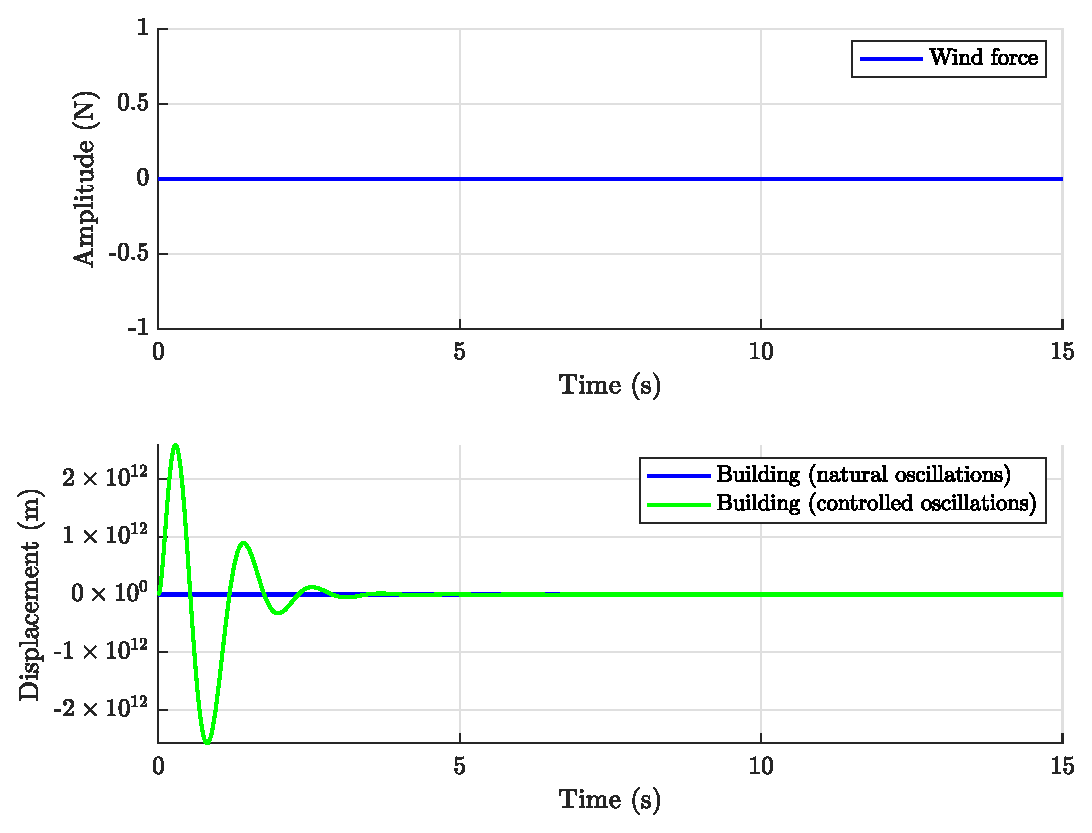
\includegraphics[width=\textwidth]{resources/eps/reference-controller.eps}
    \caption{Response to a reference variation - controlled output}
\end{figure}
\begin{figure}[H]
    \centering
    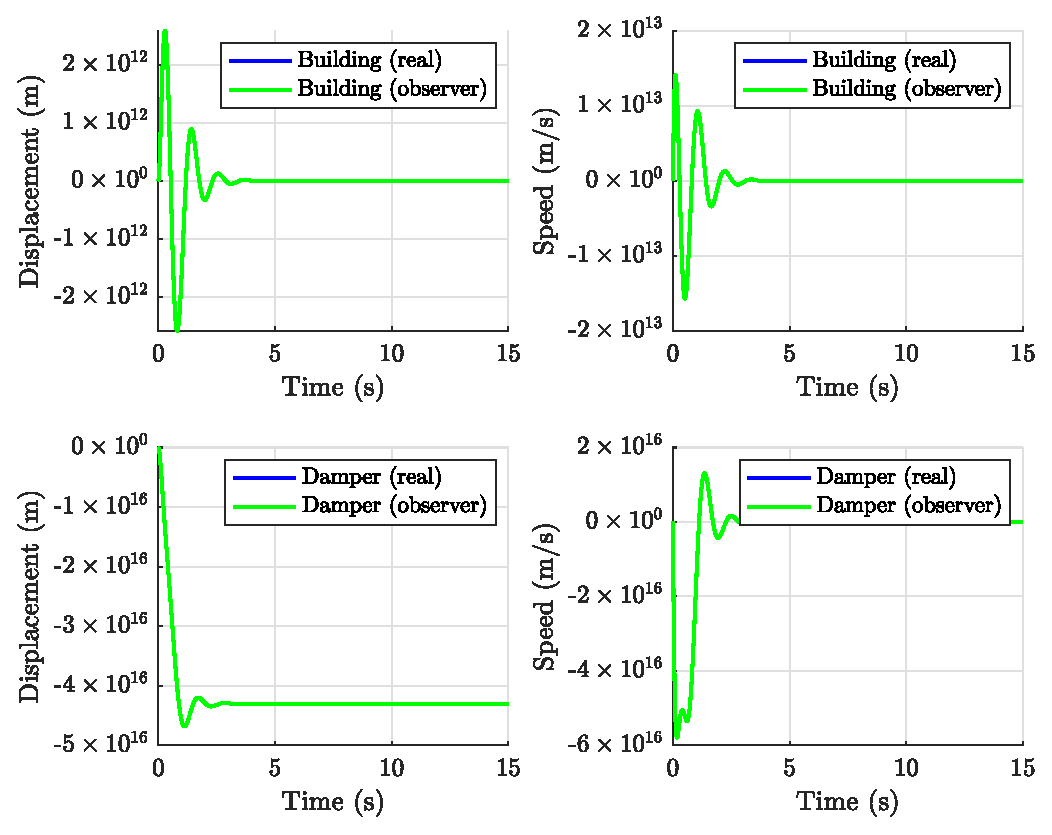
\includegraphics[width=\textwidth]{resources/eps/reference-observer.eps}
    \caption{Response to a reference variation - states}
\end{figure}

\subsubsection{Response to a perturbation (disturbance)}
For a constant wind force, we get : 
\begin{figure}[H]
    \centering
    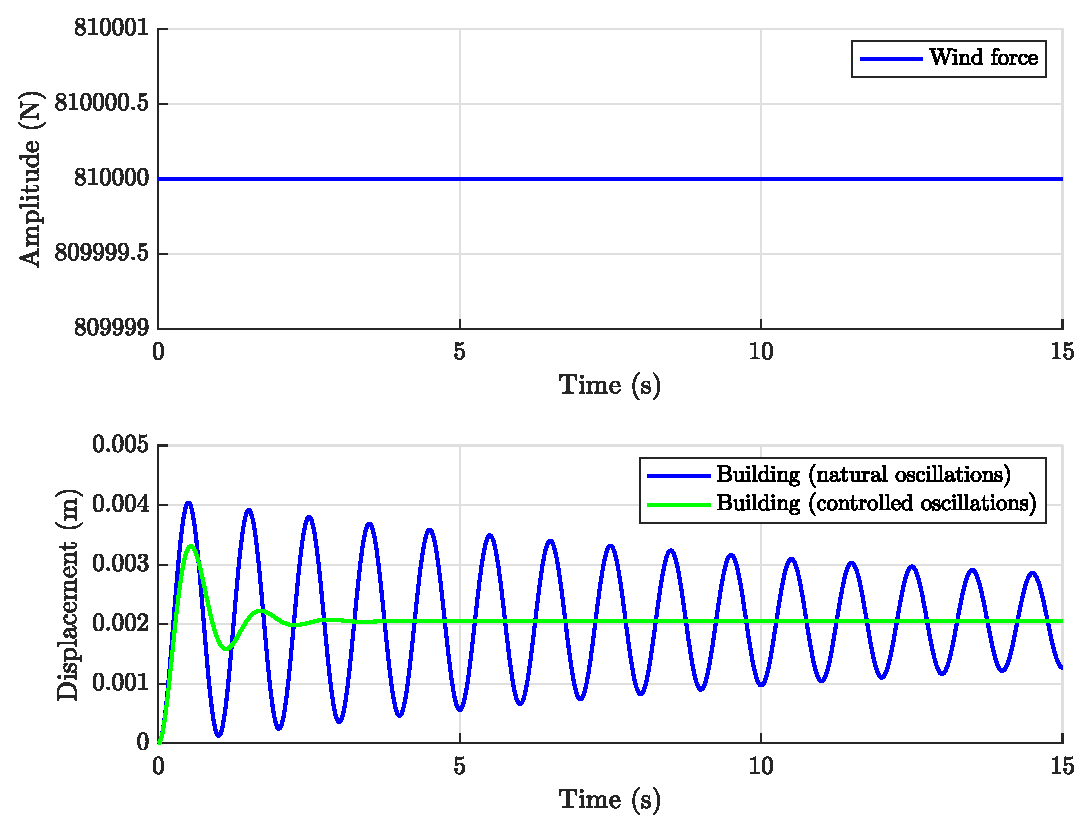
\includegraphics[width=\textwidth]{resources/eps/constant-controller.eps}
    \caption{Response to a constant wind force - controlled output}
\end{figure}
\begin{figure}[H]
    \centering
    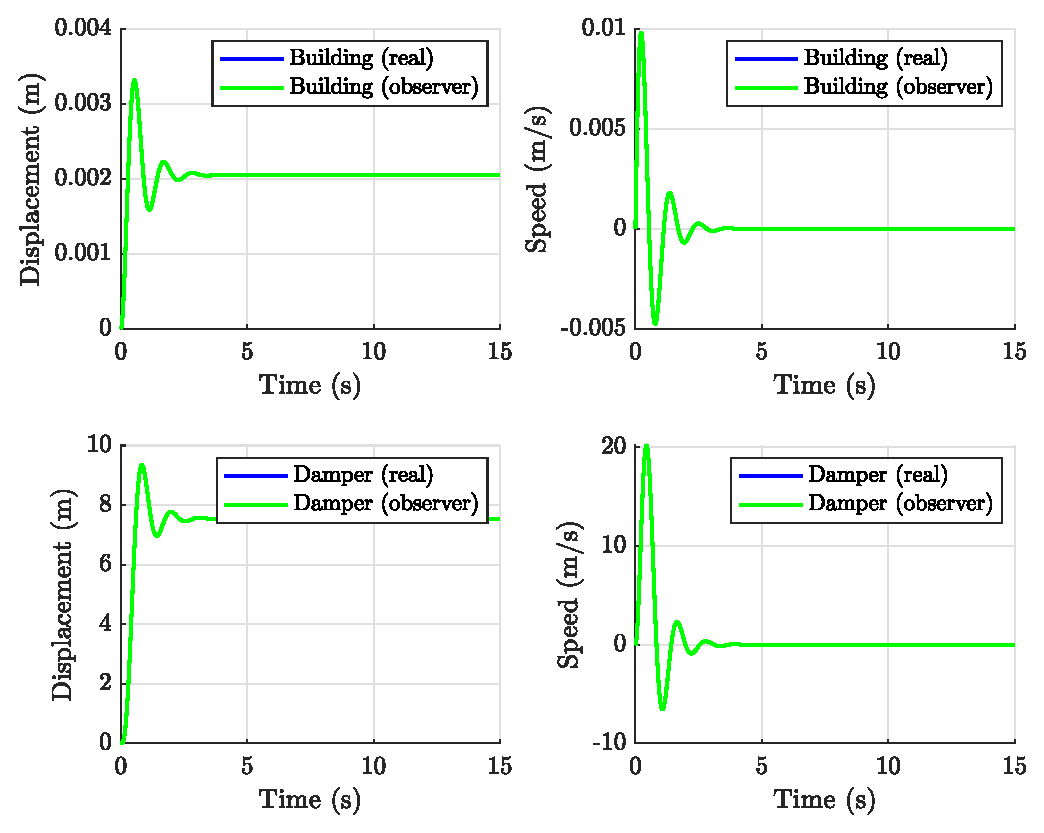
\includegraphics[width=\textwidth]{resources/eps/constant-observer.eps}
    \caption{Response to a constant wind force - states}
\end{figure}
For a sinusoidal wind force, we get : 
\begin{figure}[H]
    \centering
    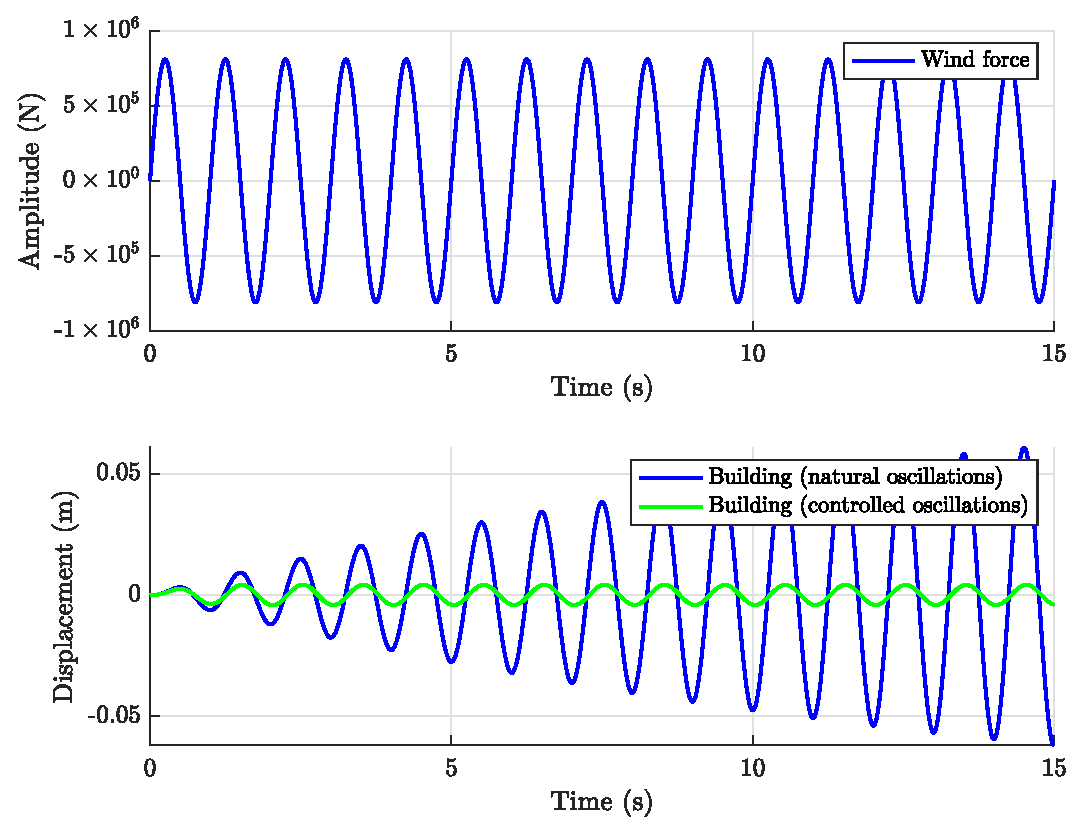
\includegraphics[width=\textwidth]{resources/eps/sinusoidal-controller.eps}
    \caption{Response to a sinusoidal wind force - controlled output}
\end{figure}
\begin{figure}[H]
    \centering
    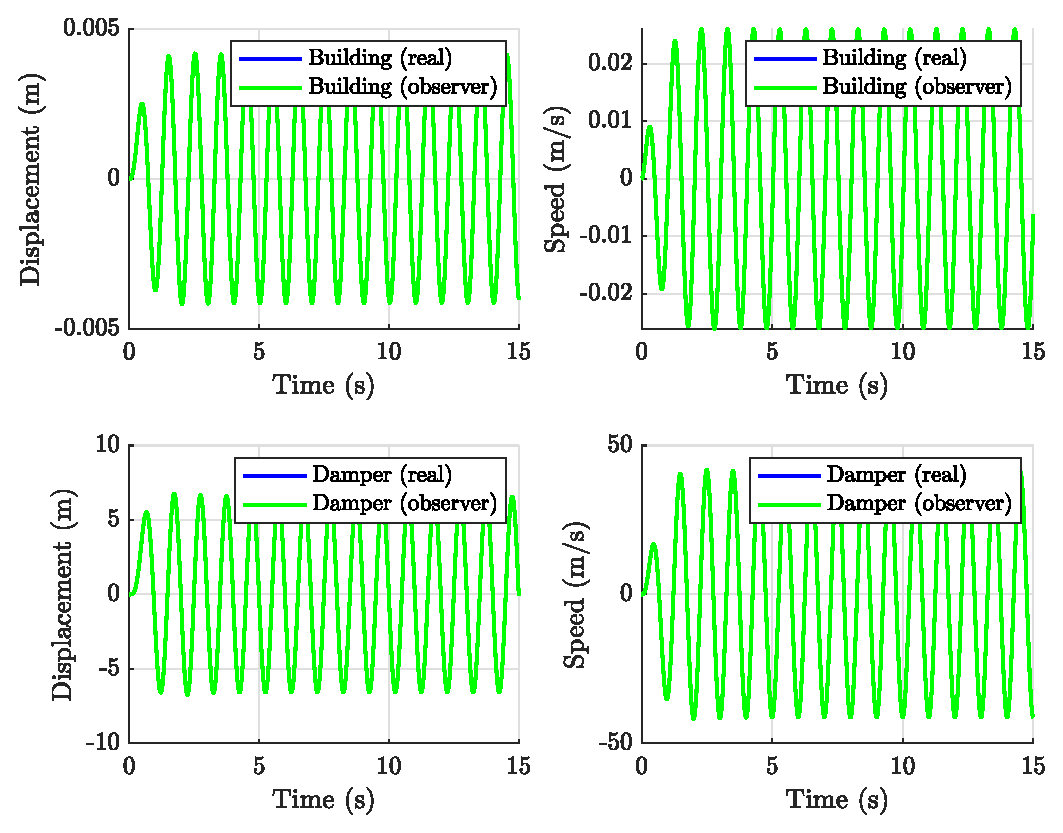
\includegraphics[width=\textwidth]{resources/eps/sinusoidal-observer.eps}
    \caption{Response to a sinusoidal wind force - states}
\end{figure}

\subsubsection{Presence of noise}
to do

\subsubsection{Impact of delays}
to do
